\documentclass[11pt,a4paper]{article}
\usepackage[utf8]{inputenc}
\usepackage[T1]{fontenc}
\usepackage[margin=2.5cm]{geometry}
\usepackage{amsmath,amssymb}
\usepackage{booktabs,array}
\usepackage{graphicx}
\usepackage{xcolor}
\usepackage{tikz}
\usetikzlibrary{arrows.meta}
\usepackage{enumitem}
\usepackage{placeins}
\usepackage[colorlinks=true,linkcolor=blue!50!black,citecolor=blue!50!black,urlcolor=blue!50!black]{hyperref}

% Markers: red = work still to do, orange = fact to check against a primary source
\newcommand{\todo}[1]{\textcolor{red}{[TODO: #1]}}
\newcommand{\verify}[1]{\textcolor{orange!80!black}{[verify: #1]}}
% Idea ledger entry: title, label, status, idea, pros, cons, next test
\newcommand{\ledger}[7]{\subsection[#1]{#1 \hfill {\small\textit{[#3]}}}\label{#2}%
\noindent\textbf{Idea.} #4\par\smallskip
\noindent\textbf{Pros.} #5\par\smallskip
\noindent\textbf{Cons and risks.} #6\par\smallskip
\noindent\textbf{Next test.} #7\par\medskip}

\title{FPGA-Native Recurrent Logic Blocks as Spiking Hidden Units\\[0.4em]\large Investigation Draft}
\author{Shamikh Al-Suwi}
\date{November 2026}

\begin{document}
\maketitle

\begin{abstract}
 Starting from the differential-time SNN architecture of Windhager et~al.\ and analyzing it in detail: claims, mechanisms, a derived cost model, evidence, strengths, weaknesses and open questions. we then collect every idea raised so far for using the FPGA's own logic block (a look-up table, a register and an output multiplexer, joined by routing feedback) as the hidden unit of a spiking network, each with pros, cons and a next test, followed by the detailed designs. Nothing here is final: ideas move between \emph{active}, \emph{parked} and \emph{rejected}, and \textbf{no experimental results exist yet}.
\end{abstract}

% Executive summary (front matter, placed before the table of contents).
\phantomsection
\addcontentsline{toc}{section}{Executive summary}
\section*{Executive summary}

\paragraph{Purpose and status.} This document is an investigation draft for a master's thesis. It states one research idea, analyzes the baseline paper it builds on, and collects the unit designs, learning methods, implementation steps and experiments needed to test the idea. No simulation or hardware result exists yet; every statement about the proposed design is reasoning, and each idea carries the status \emph{active}, \emph{parked} or \emph{rejected} (Section~\ref{sec:ledger}).

\paragraph{The idea.} The hidden layer of a spiking neural network is built from the FPGA's own logic block: a look-up table (LUT), a flip-flop and an output multiplexer, with feedback through the routing fabric (Section~\ref{sec:idea}). This is not an ordinary SNN implemented on an FPGA; the computational unit is made of the resources every logic block already contains. Two variants are considered (Section~\ref{sec:unit}): the minimal unit, a single LUT--FF--MUX block whose four truth-table bits are the learned parameters, and a cluster of several blocks with wider state and higher fan-in. Input and output layers are unrestricted, with delta encoding at the input and counters with argmax at the output; the hidden layer is the research object. Units communicate in one-bit events, hold persistent state, and update in parallel on every clock; any latency advantage over the baseline's serial scan is a design estimate, not a measurement (Section~\ref{sec:impl}).

\paragraph{Expected contribution.} Nothing is claimed yet. A contribution has to be established through a literature review and measured results, plausibly around the FPGA-native recurrent hidden unit, its state-transition structure, its resource and timing behavior, and recurrent trajectory comparison inside that structure (Section~\ref{sec:idea}). The feed-forward part has prior art in LogicNets, NeuraLUT and differentiable logic and weightless networks; the recurrent state-carrying unit with delta or differential-time coding may be the open part.

\paragraph{What the baseline gives and lacks.} The reference paper, Windhager et~al.\ (Section~\ref{sec:paper}), runs a fully connected SNN on MNIST (784--1000--10) at 97.00\% accuracy with 6-bit weights, about 838 images/s and 5.46 mJ/image on a Zynq ZCU102. Its strengths are multiplier-free arithmetic, robustness to coarse weights, and a differential-time code that decouples spike time from processing time. A derived cost model shows the limits: latency grows with fan-in times the number of distinct spike times, so pruning saves nothing; layers are processed one after another over stored spike trains, which rules out recurrence and lateral links; there is one global decay constant; and the evidence rests on a single run on static data, with training--hardware equivalence unverified and resource figures that need checking.

\paragraph{Relation to the LIF neuron.} By the strict definition the logic-block unit is not an LIF neuron (Section~\ref{sec:snnq}); it is a quantized four-state spiking unit, closest to a finite-state machine that emits spikes. What is lost, namely the weighted sum over many synapses, the graded potential with decay and the timing information, can be recovered inside the same primitives (Section~\ref{sec:recover}): a dendrite tree of branch and merge LUTs at about $n/3$ LUT4s per neuron for $n$ inputs, a wider saturating soma with a shared leak tick that replaces the decay constant, and a time replay counter that turns the differential time code into clock time.

\paragraph{Learning.} Plain backpropagation does not apply: truth-table bits have no slope, state is recurrent, and counting followed by argmax is not differentiable (Section~\ref{sec:learning}). The candidate methods are policy gradient over bit probabilities, evolutionary search in a bit-exact simulator, a reward-modulated local rule that would need writable table storage, and enumeration of a trained few-bit neuron, which gives a starting point that search can refine. Differentiable relaxations are set aside for now.

\paragraph{Change detection.} A Siamese variant runs two recurrent paths with shared tables and compares state and transition differences through a third recurrent cluster that keeps its own mismatch history (Section~\ref{sec:siamese}). It targets transient, sustained, repeated and reversed changes between two observations; it is an experimental possibility, not a proven capability.

\paragraph{Path to results.} The build order is: reproduce the baseline in snnTorch, write a bit-exact software model of the logic-block network, implement the unit in SystemVerilog and verify it against the model, add the layer structure, then load to the board and measure (Section~\ref{sec:impl}). The board is a Sipeed Tang Primer 20K; the first target is a sparse network, with the image downsampled to $14\times14$, about 100 hidden units with fan-in 16--64, and 10 output counters. The experimental plan (Section~\ref{sec:experiments}) covers temporal-pattern discrimination, synthetic change detection with paired paths, an MNIST comparison at an equal resource budget, and scaling and ablation studies; an improvement is attributed to a feature only if an ablation isolates it.

\paragraph{Main risks.} The open questions (Section~\ref{sec:open}) reduce to five risks. (i) The advantage over finite-state machines, reservoir computing and weightless networks is unproven, and the novelty claim is not yet established. (ii) A two-bit state remembers only the last change, so long dependencies need depth or lateral loops. (iii) Fan-in four and the dendrite-tree cost limit connectivity, and the right sparsity level is unknown. (iv) No candidate training method is known to scale to the number of table bits. (v) Recurrence forces clock-locked updates, which may dissolve the baseline's decoupling of spike time and processing time.

\paragraph{Idea ledger snapshot.} Of the 21 ideas collected so far, 12 are active, 7 are parked and 2 are rejected: quantum computing, and reliance on physical effects such as metastability or RC elements. Each entry carries pros, cons and a next test (Section~\ref{sec:ledger}).

\newpage

\tableofcontents

\medskip\noindent\textbf{Markers.} \textcolor{red}{[TODO]} work still to do; \textcolor{orange!80!black}{[verify]} a fact to check against a primary source; \textit{[active]}, \textit{[parked]}, \textit{[rejected]} the current status of an idea. Numbers marked ``derived'' were computed from the paper's reported values, not reported by it.
\newpage

\section{Research idea}
\label{sec:idea}
The direction is to investigate hidden neural computation built from FPGA-native logic structures, rather than implementing an ordinary SNN on an FPGA or mapping a conventional neuron onto a processor-style datapath. The computational unit is made of the resources every logic block already contains: a look-up table (LUT), a register (flip-flop, FF) and an output multiplexer (MUX), with feedback through the routing fabric. Two variants are considered (Section~\ref{sec:unit}): the minimal unit, a single LUT--FF--MUX block, and a cluster of several such blocks working together.

\paragraph{Layer roles.} Input and output layers are unrestricted and may use conventional multi-bit arithmetic (delta encoding, counters, argmax). The focus is the hidden layer, whose units are recurrent logic blocks or clusters.

\paragraph{Status of claims.} Behaviors listed in this document (temporal-pattern recognition, coincidence detection, event ordering, persistence, repeated-event detection, suppression, change direction) are hypotheses to test, not presumed advantages.

\paragraph{Novelty discipline.} Siamese comparison, recurrent dynamics, SNN temporal encoding, logic-based neural computation and change detection each have prior literature, and their combination is not itself a novelty claim. A contribution has to be established through a literature review and measured results, plausibly around the FPGA-native recurrent hidden unit, its state-transition structure, its resource and timing behavior, and recurrent trajectory comparison inside that structure. \todo{literature review: recurrent LUT-based units, Boolean networks, weightless networks, reservoir computing}

\section{Background}
\label{sec:background}

\subsection{FPGA fabric}
Island-style FPGAs consist of a grid of logic blocks, a routing fabric of wire segments joined by switch boxes and connection blocks, and I/O blocks at the edge~\cite{boutros2021,kuon2008,betz1999}. A basic logic block contains a $k$-input LUT whose output goes both to the D input of a flip-flop and directly to an output MUX; the MUX picks the combinational or the registered path (Fig.~\ref{fig:logic-block}). Dedicated carry signals link neighboring blocks. Truth tables come from the configuration bitstream, so in SRAM-based devices they are not writable as ordinary data at run time and vanish at power-off.

\subsection{The reference paper in brief}
Windhager et~al.~\cite{windhager2024} propose a lightweight SNN layer architecture for digital hardware built on delta-encoded inputs, differential spike-time coding and a LIF neuron with power-of-two decay,
\begin{equation}
P_k = r_f\!\left(P_{k-1}\,\beta^{\Delta t} + \sum_i w_i s_i\right),
\qquad
r_f(P)=
\begin{cases}
P, & \theta_{\text{low}}<P<\theta_{\text{high}}\\
P-\theta_{\text{low}}, & P\le\theta_{\text{low}}\\
P-\theta_{\text{high}}, & P\ge\theta_{\text{high}}.
\end{cases}
\label{eq:lif}
\end{equation}
Table~\ref{tab:baseline} lists the reported results. Section~\ref{sec:paper} analyzes the paper in detail.

\begin{table}[t]
\centering
\caption{Reported results of the baseline~\cite{windhager2024} (MNIST, 784--1000--10 network). Values copied from the paper.}
\label{tab:baseline}
\begin{tabular}{@{}lcc@{\qquad}lc@{}}
\toprule
Weight bits & Accuracy & & Metric & Zynq ZCU102 (this paper)\\
\midrule
4 & 95.84\% & & Max.\ clock & $\approx$365 MHz\\
5 & 96.90\% & & Clock cycles (avg.) & 435\,368\\
6 & 97.00\% & & Images/s & $\approx$838\\
7 & 97.07\% & & Energy & 5.46 mJ/image\\
8 & 97.05\% & & CLBs & 108\,894\\
9 & 97.08\% & & Registers & 57\,659\\
\bottomrule
\end{tabular}
\\[0.4em]
{\footnotesize The compared design~\cite{li2021fast} (Virtex-7 VC707) is reported at $\approx$100 MHz, 92.92\% accuracy, $\approx$320 images/s and 5.04 mJ/image.}
\end{table}

Related event-based hardware includes TrueNorth~\cite{akopyan2015} and Loihi~\cite{davies2021}; SNN surrogate-gradient training is covered by snnTorch~\cite{eshraghian2023}.

\section{Analysis of the reference paper}
\label{sec:paper}
This section analyzes Windhager, Moser and Lunglmayr~\cite{windhager2024} in detail, because every extension below is measured against it. The aim is to separate what the paper claims, what its evidence shows, and what it leaves open. Numbers in quotation of the paper are marked ``reported''; numbers computed from them are marked ``derived'' and are only as good as the assumptions stated. Open points are phrased as questions, since several may be answered by details the short conference format left out.

\subsection{Claims and contributions}
The paper states three contributions: (a) a low-complexity architecture that processes full layers of an SNN using differential time encoding of spike trains, decoupling spike time from processing time; (b) inference results on MNIST that it describes as superior to a recent state-of-the-art solution; (c) robustness to quantization, with high accuracy down to 4-bit weights. Two further claims appear in the text: the design needs no multipliers, and more than 1000 neurons fit on a moderately sized FPGA.

\subsection{Encoding}
\paragraph{What it does.} The input is delta encoded: a spike of signed amplitude is emitted when the change of the signal exceeds a threshold (0.05 in the experiment). Spike times are stored as differences $\Delta t_k=t_k-t_{k-1}$ in sign-magnitude form. Because sign-magnitude has a negative zero, an amplitude $a>1$ is written as one unit spike followed by $a-1$ spikes with $\Delta t=0$. The all-ones pattern is reserved as a timer-overflow spike that carries only the passage of time, so the width of $\Delta t$ can be chosen freely: fewer bits mean more overflow spikes.

\paragraph{Observations.}
\begin{itemize}[leftmargin=1.5em]
\item The scheme removes the growing absolute timestamp of address-event representation (AER); neuron identity is not needed either, because connections are fixed wires.
\item The trade-off between the width of $\Delta t$ and the number of overflow spikes is described but not quantified; no plot or number is given for MNIST.
\item An amplitude $a$ costs $a$ spike slots, so the processing cost of strong changes grows linearly with amplitude.
\item Delta encoding versus rate coding is motivated in the introduction but never compared in the paper's own experiments.
\end{itemize}

\subsection{Neuron model}
Equation~\eqref{eq:lif} is the event-driven LIF update: the decay $\beta^{\Delta t}$ is applied lazily at the time of the next input, with $\Delta t$ the time since the last update. With $\beta=2^{-i}$ it is a right shift by $i\,\Delta t$ bits. Reset subtracts the threshold with the sign of the spike, and because several spikes can occur at $\Delta t=0$, the reset is a modulo operation (``reset-to-mod''). An arbitrary decay is claimed to be obtainable by globally scaling all spike times by $\lambda=\log\beta/\log 2^{-i}$.

\paragraph{Observations and questions.}
\begin{itemize}[leftmargin=1.5em]
\item \emph{Time scaling.} Scaling all times by a non-integer $\lambda$ changes the time grid, the width of $\Delta t$ and the number of overflow spikes, and requires rounding; this is not discussed. A global $\lambda$ also gives all layers the same time constant, so heterogeneous time constants (useful for temporal tasks) are not available.
\item \emph{Training--hardware equivalence.} Training uses snnTorch's \texttt{LeakySurrogate} neuron in discrete time steps. The hardware updates only at event times, resets immediately and can emit several spikes at one instant. My recollection is that snnTorch derives the reset from the previous step's membrane potential and emits at most one spike per step \verify{check snnTorch implementation}. If so, the semantics differ, and the paper does not say whether the reported accuracies come from the hardware-exact model or from snnTorch with quantized weights.
\item \emph{Negative spikes.} The experiments use only a positive threshold of one, so $\theta_{\text{low}}$ and negative output spikes are not exercised.
\item The fixed threshold of one means the weight scale carries all gain; how the 4--9-bit grid is scaled relative to the threshold is not stated.
\end{itemize}

\subsection{Hardware architecture}
\paragraph{Layer structure.} Each layer is fully connected to the previous one; there are no connections inside a layer. Every neuron of the SNN maps to one physical neuron. A layer produces whole vectors of differentially encoded spike data, which the next layer consumes, so layers are processed one after another and spike trains between layers must be stored. If a network does not fit, a subnetwork is reused and intermediate spike data go to memory.

\paragraph{Common stage of a layer (Fig.~3 of the paper).} Each input synapse has a buffer, an absolute-value block and an integrator that converts differential time to absolute time $t_i$. The $n$ times are rotated $n$ times through a comparator to find the minimum, which is the time of the next incoming spike; the stage also holds the current time $t_\text{curr}$ and last time $t_\text{last}$. Integrators are reduced whenever an overflow spike is emitted, so their width stays bounded. This stage exists once per layer, because all neurons see the same inputs.

\paragraph{Neuron core (Fig.~4 of the paper).} A rotation register holds the neuron's weights and rotates in step with the common stage. When a new minimum is found, a weight accumulator restarts; spikes with the same time are added to it. The accumulated weight is added to the decayed potential (decay by shifter), the result is compared with the threshold, and an output spike is encoded relative to a last-spike-time register. No multiplier is used because spike amplitudes are integers.

\subsection{Derived cost model}
\label{sec:costmodel}
\paragraph{Latency.} Finding the next spike time takes one rotation of $n$ entries, i.e.\ $n$ clock cycles, per distinct input spike time. For a layer with $n$ inputs and $E$ distinct spike times, latency is about $nE$ cycles, independent of the number of neurons in the layer (all neurons rotate in parallel). For the 784--1000--10 network this gives $784E_1+1000E_2$ if the layers run one after another. The reported 435\,368 cycles per image would correspond to about 555 rotations if all cost were in the first layer and about 435 if all were in the second (derived: $435\,368/784$ and $435\,368/1000$). The paper gives no breakdown, so this is a hypothesis to test by counting delta events per MNIST image.

\paragraph{Consequences.}
\begin{itemize}[leftmargin=1.5em]
\item Latency scales with fan-in times the number of events, not with the number of neurons: neuron count is cheap in time and expensive in area.
\item Cutting a connection by setting its weight to zero (as the paper suggests) does not shorten the scan, since the entry is still rotated past. Sparsity saves nothing in latency in this scheme.
\item The reported 838 images/s is consistent with the cycle count (derived: $435\,368/365\,\mathrm{MHz}\approx1.19$ ms, i.e.\ $\approx838$ images/s).
\end{itemize}

\paragraph{Storage.} Hidden-layer weights alone are $784\times1000\times6\approx4.70$ Mbit and output weights about 60 kbit at 6 bits (derived). The reported 57\,659 registers are far below this, so the weights must live in block or distributed RAM; the paper reports no BRAM, LUT-RAM or DSP counts, and the storage for intermediate spike trains is not quantified.

\paragraph{Power.} Energy per image times throughput gives an implied average power of about 4.6 W for this design ($5.46\,\mathrm{mJ}\times838\,\mathrm{s^{-1}}$) and about 1.6 W for the compared design ($5.04\,\mathrm{mJ}\times320\,\mathrm{s^{-1}}$), both derived. The new design is faster but draws more power, so energy per image is not improved.

\subsection{Experimental evidence}
\paragraph{Setup (reported).} 784 inputs, 1000 hidden and 10 output neurons; the output neuron with most spikes wins; threshold one, positive spikes only; snnTorch Tutorial~5 with \texttt{LeakySurrogate}, pixels in $[0,1]$, 100 epochs; delta threshold 0.05; $\beta=0.5$; ``the spike sequence of an image is fed into the network in parallel 28 times'' (meaning unclear to me: 28 image rows, 28 time steps or 28 copies). Results are in Table~\ref{tab:baseline}.

\paragraph{Observations.}
\begin{enumerate}[leftmargin=1.5em]
\item \emph{Static data only.} MNIST images are static, and ``time'' is the pixel scan index. The central selling point, differential time with decoupled processing, is never tested on data with real temporal structure (event camera, audio, time series), although the cited prior work~\cite{moser2017,lunglmayr2021} is about sampled signals.
\item \emph{No ablation of the ingredients.} There is no comparison of delta versus rate coding, differential versus absolute time, or with and without overflow spikes. The accuracy gap to the compared design (97.00\% versus 92.92\%) may come from training, network size or precision rather than from the architecture.
\item \emph{Single run, no spread.} For a 10\,000-image test set the standard error at 97\% is about 0.17 percentage points (derived: $\sqrt{0.97\cdot0.03/10^4}$). The differences between 6 and 9 bits (97.00--97.08\%) are well inside that, so only the drop at 4 and 5 bits is clearly visible.
\item \emph{Quantization study.} Only weights are quantized, apparently after training (``running the SNNs with the quantized weights''). Whether quantization-aware training was tried, how the scale is chosen, and which accumulator and potential widths guarantee ``no further quantization effects'' are not given.
\item \emph{Like-for-like comparison.} The compared design~\cite{li2021fast} uses 16-bit floats on a Virtex-7, supports online learning, and sits on an older process generation \verify{28 nm Virtex-7 versus 16 nm UltraScale+}. How power and energy were measured, and whether on board or chip level, is not stated.
\item \emph{Resource figures.} 108\,894 ``CLBs'' cannot be CLBs for a ZCU102-class device, which has roughly a third of that many CLBs and about 274\,k LUTs \verify{vendor datasheet}; it looks like a LUT count. No breakdown into LUT, BRAM, DSP, no utilization percentage, and no statement whether 365 MHz is a target or achieved timing.
\item \emph{Latency distribution.} The cycle count is an average; since the design is event driven, it varies per image, and the worst case matters for real-time use.
\item \emph{Reproducibility.} Training hyperparameters beyond the tutorial setup and the availability of code or bitstreams are not stated.
\item \emph{Editorial.} Table~I carries the caption of Table~II.
\end{enumerate}

\subsection{Strengths}
\begin{itemize}[leftmargin=1.5em]
\item A clear, simple idea: store time differences, keep integrators bounded with overflow spikes, and let processing time run on its own clock.
\item Multiplier-free arithmetic, because inputs are integer-amplitude spikes and decay is a shift.
\item Robust to coarse weights: 95.84\% at 4 bits is a strong result for a $784\text{--}1000\text{--}10$ network.
\item A neuron count that is free in time: every neuron in a layer works in parallel on the same rotation.
\item An honest, explicit trade-off between $\Delta t$ width and overflow-spike count, and a path to subnetwork reuse for large networks.
\end{itemize}

\subsection{Limits implied by the architecture}
\begin{itemize}[leftmargin=1.5em]
\item The serial scan makes latency proportional to fan-in times event count, and sparsity does not help.
\item Layer-by-layer processing with stored spike trains rules out recurrence and lateral connections unless a global time ordering across layers is added. This directly affects the recurrent unit proposed here (Section~\ref{sec:ledger}).
\item Fully connected layers only; no convolution or weight sharing, which hurts for images.
\item One global $\beta$; no heterogeneous time constants.
\item No online learning; training is offline in software, and its equivalence to the hardware is unverified.
\end{itemize}

\subsection{Questions for discussion with the author}
\begin{enumerate}[leftmargin=1.5em]
\item Are the Table~I accuracies from bit-exact hardware simulation or from snnTorch with quantized weights? Was quantization post-training?
\item What does ``fed into the network in parallel 28 times'' mean, and how many delta spikes does an average image produce?
\item Where do the 435\,368 cycles go (layer 1, layer 2, overhead), and what are the best and worst cases?
\item Where are the weights stored, and what are the LUT, BRAM and DSP counts? What does the ``CLBs'' entry count?
\item How were energy and power obtained (measured on board, estimated by the tool, which parts included)?
\item What accumulator and potential widths were used, and what do narrower ones cost in accuracy?
\item Were rate coding and absolute-time coding ever compared in the same network?
\item How does the design behave on data with real temporal structure?
\item How does the training model's reset and spike semantics match the hardware's reset-to-mod?
\item Can the scan be replaced by a faster minimum search without losing the decoupling?
\item Is a per-layer or per-neuron decay practical with the time-scaling argument?
\item Are code, bitstreams or RTL available for reproduction?
\end{enumerate}

\subsection{Directions the paper opens}
\begin{enumerate}[leftmargin=1.5em]
\item Reproduce the result and verify the cost model by counting delta events per image.
\item Extend Table~I below 4 bits and to the membrane potential.
\item Replace the rotation with a faster next-event search (parallel minimum tree, sorted event queue, time wheel) and measure the cycle count.
\item Fan out events directly (AER-style: look up the targets of each spike) so that pruned weights save time; compare with the scan for sparse spike trains.
\item Evaluate on temporal datasets (event camera, audio, ECG) where decoupled time should matter.
\item Allow per-layer decay and test the time-scaling argument.
\item Recurrence through a global event queue.
\item Enumerate a few-bit neuron core into LUT contents (Section~\ref{sec:ledger}).
\end{enumerate}

\section{Idea ledger}
\label{sec:ledger}
Every idea raised so far, with pros, cons and a next test. Status tags are provisional: an idea can move between \emph{active}, \emph{parked} and \emph{rejected} as evidence comes in. Details of the designs follow in later sections.

\ledger{Logic block (LUT--FF--MUX) as the hidden neuron}{idea:block}{active}
{Use the logic block itself as a recurrent unit: the LUT sees a new input bit and the unit's own previous output, the FF stores the state, the MUX selects the registered path (Sec.~\ref{sec:unit}). The four rows of $(x_1,x_2)$ are the change between old and new bit; the four stored bits are what is learned.}
{Smallest possible unit: one LUT and one FF. Maps onto the fabric without arithmetic, so many units fit and timing is short. Every unit updates in parallel on each clock. Only 16 possible functions, which makes exhaustive analysis possible.}
{Fan-in of four limits what one unit sees; one or two state bits give coarse memory; no graded weights or potential; LUT contents are fixed by the bitstream, so on-chip learning needs extra writable storage. Accuracy on non-trivial tasks is unknown. Feed-forward LUT networks already exist (Sec.~\ref{idea:prior}).}
{Bit-exact software model of one layer on synthetic temporal patterns (Sec.~\ref{sec:experiments}); then MNIST for reference.}

\ledger{Change-state encoding (low, falling, rising, high)}{idea:states}{active}
{Read the two-bit state, or the row index, as the change between old and new input rather than a value. Stable low and stable high are the saturated states; rising and falling are transitions.}
{Matches an edge detector or up/down saturating counter; natural for temporal signals; fits the delta-coded input of the paper.}
{The hidden layer repeats what the delta encoder already does at the input; a two-bit state remembers only the last change, so long dependencies need depth or feedback. Encoding is a free design variable and the proposed one may not be the best.}
{Compare against Gray, one-hot and learned encodings at equal bits; check whether it beats a plain two-bit counter.}

\ledger{Cluster of LUTs, dendrite tree and merge}{idea:cluster}{active}
{A unit made of several branch LUTs, state LUTs, registers and muxes (Variant B). Dendrite LUT4s vote over four spikes each; merge LUT4s combine them; a soma block holds the state (Sec.~\ref{sec:recover}).}
{Raises fan-in beyond four; branches are learned local nonlinearities; dendrite and merge blocks are stateless and can be combinational.}
{About $n/3$ LUT4s per neuron for $n$ inputs: a 784-input neuron costs about 260 LUT4s and does not scale on small devices. Combinational depth lowers Fmax unless registered. Ternary weights only.}
{Synthesize one neuron with 16, 64 and 256 inputs; record LUTs and Fmax; check accuracy against sparse versus dense connections.}

\ledger{Complex multi-bit input and output layers}{idea:io}{active}
{Keep input and output layers unrestricted: delta, thermometer or sigma-delta encoding at the input; counters, adder trees and argmax at the output; the hidden layer is the research focus.}
{Puts complexity where arithmetic is cheap and useful; makes the hidden layer the clean object of study; carry chains suit counting.}
{The multi-bit layers may dominate area and hide the benefit of the hidden layer; fair comparisons must count them.}
{Report resource use per layer separately.}

\ledger{Differential time and time replay at the input}{idea:replay}{active}
{Keep the paper's differential time code at the input and add a time replay counter that loads $\Delta t$, counts down and emits the spike at zero, so timing becomes clock timing; a global clock-enable or fast-forwarded leak ticks recover the decoupling.}
{Reuses the paper's bounded-width time representation; keeps spike time independent of processing time.}
{Adds a counter per input; clock-locked hidden units cannot hold the paper's layer-sequential model; fast-forwarding many ticks costs cycles.}
{Measure cycles versus Fmax for time replay against free-running clock-locked coding.}

\ledger{Leak tick and wider soma state}{idea:leak}{active}
{Widen the soma to an up/down saturating counter and add a shared slow tick that moves the state toward rest, so the tick period replaces the decay constant $\beta$.}
{Restores a graded potential and leak using the same primitives; time constant is a single shared knob.}
{More than four levels needs LUT5-sized functions on devices with only LUT4; one global tick gives one time constant for all units.}
{Sweep state width and tick period on the temporal patterns.}

\ledger{Enumerating a trained few-bit neuron into LUT contents}{idea:enumerate}{active}
{Limit the paper's neuron to a few-bit potential and small fan-in, train it with surrogate gradients as the paper does, then tabulate its update function into the truth table. The LUT becomes the neuron by construction. Emerged from the review of the paper.}
{Keeps the paper's training pipeline and delta coding; no arithmetic in the neuron; gives a trained starting point for later search.}
{A trained network needs few-bit potential and small fan-in, which may cost accuracy; surrogate-gradient training is a gradient method, which conflicts with the preference for non-gradient learning.}
{Sweep potential bits (1--4) and fan-in (2--6) in snnTorch and record accuracy against the paper's Table~I.}

\ledger{Training by reinforcement, evolution or a reward-modulated rule}{idea:rl}{active}
{Learn table bits and wiring from a score, using REINFORCE on bit probabilities, evolutionary search in a bit-exact simulator, or a local rule with one global reward (Sec.~\ref{sec:learning}).}
{Needs no gradient; matches the hardware exactly; a local rule could run on chip.}
{High variance and a huge search space with one global reward; the cost grows with the number of bits; a local rule needs writable tables.}
{Run search on a ${\sim}100$-unit network, from scratch and from the enumerated solution, and compare sample counts.}

\ledger{Differentiable relaxation of tables}{idea:diff}{parked}
{Replace tables by soft functions of probabilities and train by gradient descent, as in differentiable logic-gate networks.}
{Proven for feed-forward logic networks; efficient with GPUs.}
{The author prefers non-gradient learning; recurrent state with independence assumptions drifts from the hard network; not pursued.}
{Revisit only if search fails.}

\ledger{Stochastic spiking with an LFSR, and random-address LUT weights}{idea:stoch}{parked}
{Treat a stored $w$-bit value as a firing probability $w/2^w$ by comparing with a shared LFSR; or feed random bits to the LUT address so that the popcount of stored bits is the weight (five levels for four rows).}
{Cheap in logic; gives graded effective weights from bits; noise can regularize and helps stochastic rounding for learning.}
{Needs more time steps for the same accuracy (variance shrinks as $1/T$); LFSR correlation between units can bias results; popcount gives redundant patterns with identical weight.}
{Compare error against a deterministic counter at equal time steps.}

\ledger{Quantum computing}{idea:quantum}{rejected}
{Add quantum amplitudes or quantum computing to the LUT neuron.}
{None for this hardware.}
{On an FPGA it is only a simulation of amplitudes, which needs more bits and multipliers, the opposite of what a LUT-based network is for.}
{None.}

\ledger{Physical effects: metastability, ring-oscillator jitter, RC and input-buffer threshold}{idea:physical}{rejected}
{Use the chip's own electrical behavior as probabilistic or threshold elements: a flip-flop sampled at the edge of its setup window, ring oscillators as pacemakers or noise sources, an RC on a pin as a membrane and the input buffer as comparator, glitches as coincidence detectors, shared supply droop as coupling.}
{Biological analogies are tempting; some cost almost no logic.}
{Behavior depends on temperature, voltage and each chip; the toolchain fights metastability and loops; RC needs external parts; results would not reproduce. Per the research notes none should be relied on as a computation mechanism; at most ring oscillators serve as a noise source for random bits.}
{None planned.}

\ledger{Primitive-level mappings on the fabric}{idea:primitives}{parked}
{Map biological parts onto device primitives: carry chain as membrane integrator, distributed RAM as a writable truth table (plastic dendrite), LUT5--LUT8 mux stages as dendritic tree, asynchronous reset as refractory period, clock enable as sparsity or neuromodulation, latches and loops as unclocked neurons.}
{Closest to the hardware; several parts (carry chain, distributed RAM) are available even on small devices.}
{Vendor-specific; asynchronous and loop structures fight the timing tools; distributed RAM costs logic.}
{Pick carry-chain integrator and distributed-RAM table for a small prototype.}

\ledger{Other devices and hard blocks as analogies}{idea:hardblocks}{parked}
{Accumulator with pattern detect (DSP) as soma, shift-register LUTs as axonal delay, dual-port block RAM as synapse matrix, clock managers and input delay taps for time constants and latency coding, on-chip ADC and temperature sensing for homeostasis, partial reconfiguration for structural plasticity, flash versus SRAM configuration as long- versus short-term memory, hard CPU as neuromodulator (Appendix~\ref{app:brainstorm}).}
{Many map directly to biological functions; available on mainstream families.}
{Needs a new board; features differ by vendor and part; each adds complexity before the basic unit is proven.}
{Revisit after the board decision (Sec.~\ref{idea:board}).}

\ledger{State-dependent receptive field}{idea:rf}{parked}
{The unit's state drives muxes that choose which inputs or branches it reads next.}
{Dynamic selection could replace fixed fan-in at equal resources.}
{Adds mux logic and routing; may only add complexity; hard to train.}
{Ablation: static versus state-selected inputs at equal LUT budget.}

\ledger{Siamese paired paths and a recurrent comparison cluster}{idea:siamese}{parked}
{Two recurrent paths with shared tables compare states and transitions; a third cluster keeps mismatch history (Sec.~\ref{sec:siamese}).}
{Natural for change detection; sharing is free in hardware (same configuration).}
{Not grounded in the paper; training shared recurrent tables is unsolved; a mismatch-fed LIF neuron or counter is the baseline it must beat.}
{Synthetic change-detection suite against that baseline.}

\ledger{Recurrence and lateral links versus the paper's layer model}{idea:recurrence}{active}
{A neighbor's output into $x_3/x_4$, or feedback across layers.}
{Real recurrent dynamics inside a layer; the paper has none.}
{The paper processes layers one after another over stored spike trains, which cannot host feedback; recurrence needs a global time order (clock-locked updates or a global event queue), which may dissolve the paper's decoupling.}
{Compare clock-locked recurrence with the paper's layer-sequential model on a task that needs memory.}

\ledger{Sparse versus full connectivity}{idea:sparse}{active}
{Give each unit a small, chosen set of inputs.}
{Required by fan-in four; saves area; physically local wiring is cheaper.}
{The paper's scan gains nothing from sparsity; sparse networks can lose accuracy; choosing the wiring is a search problem.}
{Accuracy versus fan-in on MNIST and on temporal patterns.}

\ledger{On-chip learning and writable tables}{idea:online}{parked}
{Change table bits at run time.}
{Adaptation without a host.}
{Normal LUT contents are fixed by the bitstream; writable storage (registers or distributed RAM) multiplies cost; partial reconfiguration is device-specific.}
{Measure the cost of a registered table against a LUT.}

\ledger{Prior art: LUT, weightless and Boolean networks}{idea:prior}{active}
{Place the idea against differentiable logic-gate networks~\cite{petersen2022}, differentiable weightless networks~\cite{bacellar2024}, LogicNets~\cite{umuroglu2020} and NeuraLUT~\cite{andronic2024}, and against Boolean networks, finite-state machines and reservoir computing.}
{Shows what is borrowed and what could be new; the state-carrying recurrent unit with delta/differential-time coding may be the open part.}
{The feed-forward part is not new; the recurrent part may also have prior art that I have not found.}
{\todo{systematic literature search before any novelty claim}}

\ledger{Board choice}{idea:board}{active}
{Stay on the Tang Primer 20K (GW2A-18C) for LUT-level work, or buy a board with DSP accumulators, shift-register LUTs, dual-port RAM, clock managers, delay taps, ADC and partial reconfiguration, such as an Artix-7 or Zynq-7000 board.}
{The Tang 20K is available now and fully sufficient for the unit and small networks; a richer board enables the analogies above.}
{The 20K cannot hold the paper's 1000-neuron network; a new board adds cost and a different toolchain.}
{Decide after the first synthesis results show which resources are the bottleneck.}

\section{The recurrent logic unit}
\label{sec:unit}

\subsection{Variant A: one logic block}
Fig.~\ref{fig:logic-block} shows the unit. The LUT has four input wires $x_1,\dots,x_4$. In the hidden layer the MUX selects the register output, so the block output $y$ is the stored state, and $y$ is routed back to one LUT input. With $x_1$ the incoming spike bit and $x_2=y$ the unit's own previous output, the next state is
\begin{equation}
y_{t+1} = T\bigl[x_{1,t},\,y_t,\,x_{3,t},\,x_{4,t}\bigr],
\end{equation}
where $T$ is the truth table. With $x_3,x_4$ unused, $T$ has four rows, i.e.\ four learned bits and $2^4=16$ possible units. The row index is the change between old and new bit (Table~\ref{tab:rows}); the stored bit says what the unit does in response.

\begin{table}[t]
\centering
\caption{Rows of the two-input unit. $x_1$ is the new input bit, $x_2=y$ the previous output; the last column lists the four learned bits (rows $00,01,10,11$) for four example behaviors.}
\label{tab:rows}
\begin{tabular}{@{}cll@{\qquad}ll@{}}
\toprule
$x_1x_2$ & Meaning of the row & & Example unit & Stored bits\\
\midrule
00 & stays low & & follower ($y=x_1$) & 0\,0\,1\,1\\
01 & falling & & hold ($y=x_2$) & 0\,1\,0\,1\\
10 & rising & & latch high ($x_1\lor x_2$) & 0\,1\,1\,1\\
11 & stays high & & toggle ($x_1\oplus x_2$) & 0\,1\,1\,0\\
\bottomrule
\end{tabular}
\end{table}

\paragraph{MUX modes.} With the MUX on $Q$ the block is a clocked state machine, which is the hidden-layer use. With the MUX on the LUT output the block is stateless; such a block must never be fed back into itself, because that would form a combinational loop with no clock. The free inputs $x_3,x_4$ can carry two more upstream spikes or a leak tick (Section~\ref{sec:recover}).

\subsection{Variant B: logic cluster}
A cluster contains several LUTs that process subsets or combinations of signals, state logic that combines their outputs, registers that retain state, muxes that select or route signals, and recurrent feedback. A LUT is a component of the cluster, not necessarily the neuron itself. A general abstraction is
\begin{equation}
s_{t+1} = F\bigl(s_t,\, b_1(x_t),\dots,b_K(x_t),\, q_t\bigr),
\end{equation}
where $s_t$ is the internal state, $b_i$ are branch LUT functions and $q_t$ are selected or routed signals. The output may be a spike, a state-change signal, a transition code or a multi-bit state, depending on the experiment. This is a conceptual starting point, not a finalized neuron definition. Variant A is the case $K=1$ with a two-bit state. \todo{decide which variant is the primary unit of the paper}

\paragraph{State representation.} An illustrative two-bit encoding is 00 stable/low, 01 falling, 10 rising, 11 stable/high. State semantics and bit encoding are separate design variables; Gray, one-hot or learned encodings, and interpretations such as phase, event history or persistence, are all to be explored.

\paragraph{State-dependent receptive field.} The current state can drive muxes that choose which incoming signals or branch functions the cluster examines at the next update, so the unit does not evaluate a fixed input subset every cycle. This has to be compared with static selection under equal hardware budgets.

\subsection{Layers}
Fig.~\ref{fig:architecture} shows the proposed network.
\begin{description}[leftmargin=1.5em,style=nextline]
\item[Input layer (multi-bit).] A delta encoder keeps the previous sample, subtracts and compares with a threshold, emitting signed events on two wires (up, down) per input. Alternatives are thermometer coding (bit $i$ is $x>\tau_i$, so a level crossing becomes a rise or fall in the unit watching that level) and sigma-delta coding (a one-bit stream whose average is the value). A time replay counter reproduces the differential-time code of~\cite{windhager2024} in clock time (Section~\ref{sec:recover}).
\item[Hidden layers (logic blocks).] Rows of units as in Fig.~\ref{fig:logic-block}. Connectivity is set by place-and-route through the switch boxes, so wiring is chosen when the design is built. Each layer adds one clock of delay.
\item[Output layer (multi-bit).] Counters tally the spikes of each class unit over $T$ steps and the largest count wins; alternatively an up/down counter reconstructs a value from rise and fall events. Carry chains suit both.
\end{description}

\paragraph{Relation to the paper's layer model.} The baseline processes one layer after another over stored spike trains. Clock-locked recurrent units cannot be hosted by that scheme; Section~\ref{sec:ledger} (recurrence) discusses what to keep, drop or replace.

\begin{figure}[!htbp]
\centering
\resizebox{0.9\linewidth}{!}{%
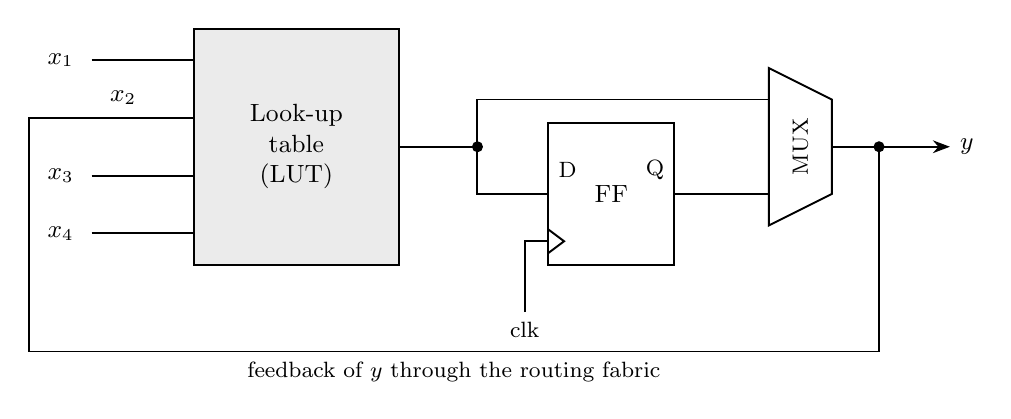
\begin{tikzpicture}[font=\small,>=Stealth,line width=0.7pt]
% LUT
\node[draw,fill=black!8,minimum width=2.6cm,minimum height=3cm,align=center] (lut) at (0,0) {Look-up\\table\\(LUT)};
% inputs x1, x3, x4 from the layer below / neighbours
\foreach \yy/\lab in {1.1/x_1,-0.37/x_3,-1.1/x_4}{
  \node[anchor=east] at (-2.7,\yy) {$\lab$};
  \draw (-2.6,\yy) -- (-1.3,\yy);
}
% x2 is the feedback wire
\node at (-2.2,0.62) {$x_2$};
\draw (7.4,0) -- (7.4,-2.6) -- (-3.4,-2.6) -- (-3.4,0.37) -- (-1.3,0.37);
\node[font=\footnotesize,anchor=north] at (2.0,-2.6) {feedback of $y$ through the routing fabric};
% LUT output
\draw (1.3,0) -- (2.3,0);
\fill (2.3,0) circle (2pt);
% bypass to MUX
\draw (2.3,0) -- (2.3,0.6) -- (6.0,0.6);
% FF
\draw (2.3,0) -- (2.3,-0.6) -- (3.2,-0.6);
\node[draw,minimum width=1.6cm,minimum height=1.8cm] (ff) at (4.0,-0.6) {FF};
\node[anchor=west,font=\footnotesize] at (3.2,-0.3) {D};
\node[anchor=east,font=\footnotesize] at (4.8,-0.3) {Q};
\draw (4.8,-0.6) -- (6.0,-0.6);
% clock
\draw (2.9,-2.1) -- (2.9,-1.2) -- (3.2,-1.2);
\draw (3.2,-1.05) -- (3.4,-1.2) -- (3.2,-1.35);
\node[font=\footnotesize,anchor=north] at (2.9,-2.1) {clk};
% MUX
\draw (6.0,1.0) -- (6.0,-1.0) -- (6.8,-0.6) -- (6.8,0.6) -- cycle;
\node[rotate=90,font=\footnotesize] at (6.4,0) {MUX};
\draw (6.8,0) -- (7.4,0);
\fill (7.4,0) circle (2pt);
\draw[->] (7.4,0) -- (8.3,0) node[right] {$y$};
\end{tikzpicture}}
\caption{Logic block used as a recurrent unit (schematic redrawn after the generic LUT--FF--MUX logic cell). The MUX selects the registered path $Q$; the block output $y$ is routed back to LUT input $x_2$, so the LUT sees the new input bit $x_1$ together with the unit's own previous output.}
\label{fig:logic-block}
\end{figure}

\begin{figure}[!htbp]
\centering
\resizebox{0.95\linewidth}{!}{%
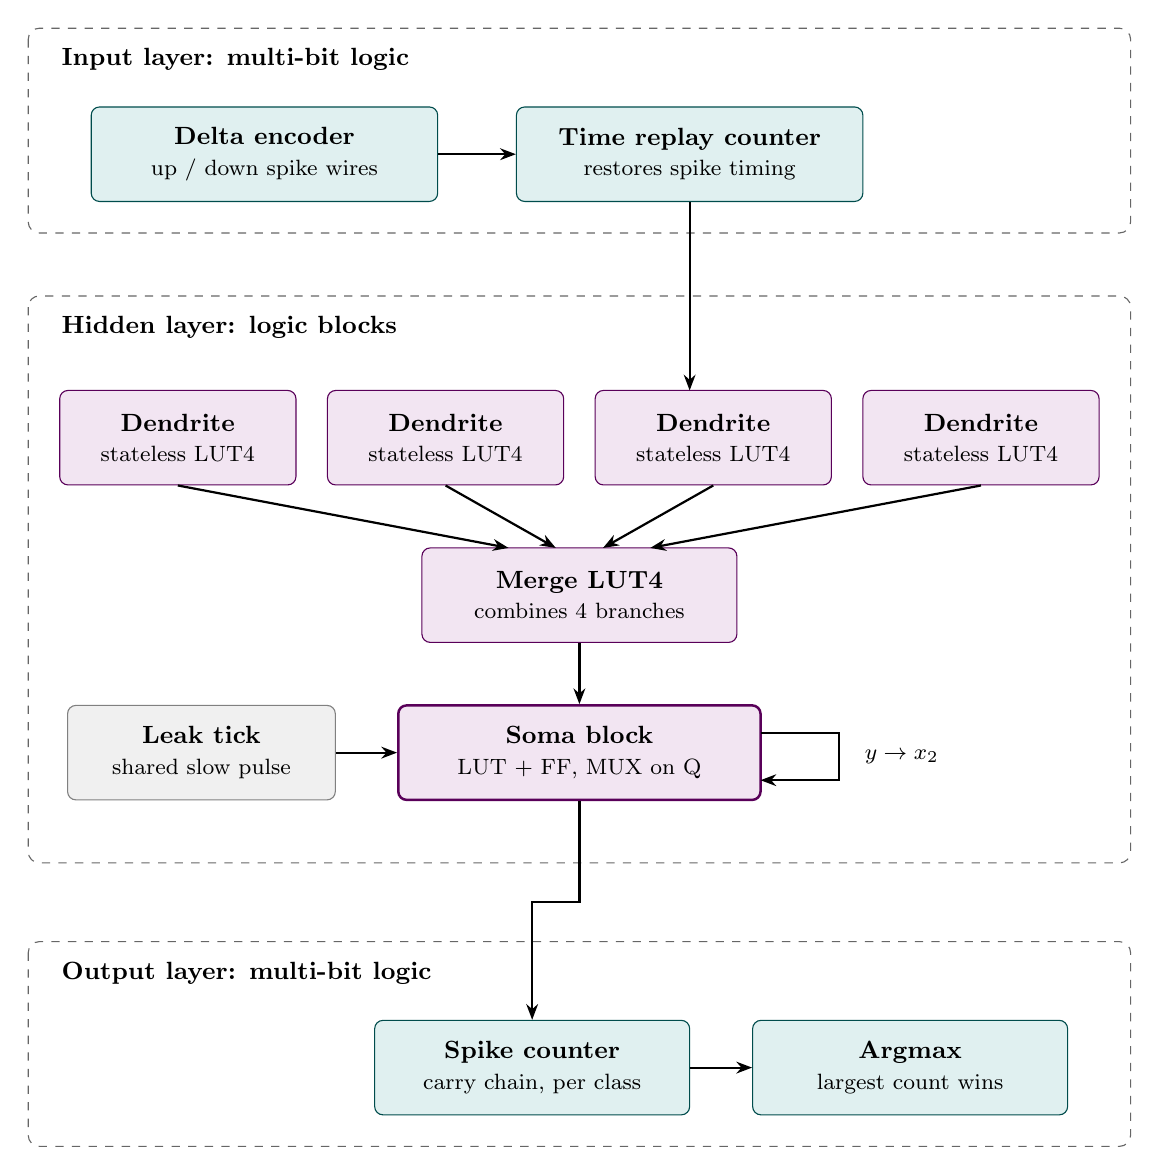
\begin{tikzpicture}[
  font=\small,
  >=Stealth,
  cont/.style={draw,dashed,rounded corners=4pt,black!60},
  tealbox/.style={draw=teal!60!black,fill=teal!12,rounded corners=3pt,align=center,minimum height=1.2cm},
  purpbox/.style={draw=violet!70!black,fill=violet!10,rounded corners=3pt,align=center,minimum height=1.2cm},
  greybox/.style={draw=black!50,fill=black!6,rounded corners=3pt,align=center,minimum height=1.2cm},
  arr/.style={-{Stealth[length=2mm]},thick}
]
% ---------------- input layer
\draw[cont] (0,0) rectangle (14,-2.6);
\node[anchor=west,font=\small\bfseries] at (0.3,-0.4) {Input layer: multi-bit logic};
\node[tealbox,minimum width=4.4cm] (enc) at (3.0,-1.6) {\textbf{Delta encoder}\\{\footnotesize up / down spike wires}};
\node[tealbox,minimum width=4.4cm] (rep) at (8.4,-1.6) {\textbf{Time replay counter}\\{\footnotesize restores spike timing}};
\draw[arr] (enc.east) -- (rep.west);
% ---------------- hidden layer
\draw[cont] (0,-3.4) rectangle (14,-10.6);
\node[anchor=west,font=\small\bfseries] at (0.3,-3.8) {Hidden layer: logic blocks};
\foreach \x/\n in {1.9/d1,5.3/d2,8.7/d3,12.1/d4}{
  \node[purpbox,minimum width=3.0cm] (\n) at (\x,-5.2) {\textbf{Dendrite}\\{\footnotesize stateless LUT4}};
}
\node[purpbox,minimum width=4.0cm] (mrg) at (7,-7.2) {\textbf{Merge LUT4}\\{\footnotesize combines 4 branches}};
\node[purpbox,minimum width=4.6cm,line width=0.9pt] (soma) at (7,-9.2) {\textbf{Soma block}\\{\footnotesize LUT + FF, MUX on Q}};
\node[greybox,minimum width=3.4cm] (tick) at (2.2,-9.2) {\textbf{Leak tick}\\{\footnotesize shared slow pulse}};
\draw[arr] (rep.south) -- (8.4,-4.6);
\draw[arr] (d1.south) -- (6.1,-6.6);
\draw[arr] (d2.south) -- (6.7,-6.6);
\draw[arr] (d3.south) -- (7.3,-6.6);
\draw[arr] (d4.south) -- (7.9,-6.6);
\draw[arr] (mrg.south) -- (soma.north);
\draw[arr] (tick.east) -- (soma.west);
\draw[arr] (9.3,-8.95) -- (10.3,-8.95) -- (10.3,-9.55) -- (9.3,-9.55);
\node[anchor=west,font=\footnotesize] at (10.5,-9.25) {$y\rightarrow x_2$};
% ---------------- output layer
\draw[cont] (0,-11.6) rectangle (14,-14.2);
\node[anchor=west,font=\small\bfseries] at (0.3,-12.0) {Output layer: multi-bit logic};
\node[tealbox,minimum width=4.0cm] (cnt) at (6.4,-13.2) {\textbf{Spike counter}\\{\footnotesize carry chain, per class}};
\node[tealbox,minimum width=4.0cm] (arg) at (11.2,-13.2) {\textbf{Argmax}\\{\footnotesize largest count wins}};
\draw[arr] (cnt.east) -- (arg.west);
\draw[arr] (soma.south) -- (7,-11.1) -- (6.4,-11.1) -- (cnt.north);
\end{tikzpicture}}
\caption{Block architecture. The input and output layers use multi-bit logic. The hidden layer uses only LUT/FF/MUX blocks: stateless dendrite and merge LUTs (MUX on the LUT output) feed a soma block (MUX on the registered output) with self-feedback and a shared leak tick. Lateral links between somas are not drawn.}
\label{fig:architecture}
\end{figure}


\begin{table}[t]
\centering
\caption{Baseline~\cite{windhager2024} versus the proposed hidden layer.}
\label{tab:compare}
\small
\begin{tabular}{@{}p{3.1cm}p{5.7cm}p{5.7cm}@{}}
\toprule
Aspect & Windhager et al. & This work\\
\midrule
Hidden unit & LIF: multi-bit potential, shifter decay, adder, comparator & LUT--FF(--MUX) state machine\\
Parameters & 4--6-bit weights rotated through one shared datapath per layer & truth-table bits and wiring\\
Next-spike-time stage & common stage per layer & none: all units update every clock\\
Time handling & differential time code, processing decoupled from spike time & clock-locked; decoupling restorable (Sec.~\ref{sec:recover})\\
Connectivity & fully connected, no links inside a layer & sparse fan-in; lateral and recurrent links possible\\
Readout & spike count, largest wins & same\\
Training & surrogate gradient (snnTorch) & open (Sec.~\ref{sec:learning})\\
\bottomrule
\end{tabular}
\end{table}

\FloatBarrier

\section{Is the unit still a spiking neuron?}
\label{sec:snnq}
It depends on how strict the definition is. What remains spiking: units communicate with one-bit events on wires in discrete time (one clock is one step); each unit has persistent internal state; activity is driven by change, so a constant input produces no events; and the output is read as spike counts. Table~\ref{tab:lif} maps the LIF ingredients of the baseline onto Variant A.

\begin{table}[t]
\centering
\caption{LIF ingredients and their counterparts in the logic-block unit (Variant A).}
\label{tab:lif}
\begin{tabular}{@{}p{4.2cm}p{9.5cm}@{}}
\toprule
LIF~\cite{windhager2024} & Logic-block unit\\
\midrule
Membrane potential & two state bits in the FF (four levels)\\
Threshold & truth-table rows that drive the state to the firing state\\
Leak & rows that return the state toward rest (needs a tick input, Sec.~\ref{sec:recover})\\
Refractory behavior & state sequence after firing (peak, falling, rest)\\
Spike & $y=1$ in the firing state\\
Reset & state transition after firing\\
\bottomrule
\end{tabular}
\end{table}

What is lost: a weighted sum over many synapses (fan-in is four per LUT), a graded potential with decay constant $\beta$, and the timing information $\Delta t$. By the strict definition (integrate weighted inputs, leak, cross a threshold, reset), Variant A is therefore not an LIF neuron. It is a quantized four-state spiking unit, closest to a finite-state machine that emits spikes. Whether the name matters is secondary to whether the network classifies well, which is untested. The next section shows how the losses are recovered inside the same primitives.

\section{Recovering what is lost}
\label{sec:recover}

\subsection{Weighted sum over many synapses: dendrite tree}
Each dendrite LUT4 is a small weighted vote over four spikes; the weights live in its table (each input counted $+1$, $-1$ or $0$, i.e.\ ternary weights). Merge LUT4s combine four branches each, and the dendrite-then-merge pattern repeats until all inputs are covered; 784 inputs need about five levels ($4^5=1024$). Dendrite and merge blocks use the MUX on the LUT output and are stateless; only the soma uses the MUX on $Q$. Registering every second level keeps the combinational path short.

\paragraph{Cost.} A tree with fan-in four needs about $n/3$ LUT4s for $n$ inputs, so one neuron with 784 inputs costs roughly 260 LUT4s. On a device with about 20.7\,k LUT4 \verify{Tang Primer 20K, GW2A-18} a fully connected 100-neuron layer does not fit; each neuron should see a sparse subset (for example 16--64 inputs), or the image should be downsampled first. For graded weights, the tree can be replaced by the accumulator of~\cite{windhager2024} on the carry chain.

\subsection{Graded potential and decay: wider soma and leak tick}
The soma state can be widened from the four change states to an up/down saturating counter (still one LUT and one FF per state bit); more than four levels need LUT5 functions, built from two LUT4s and the slice mux \verify{check the vendor documentation for the target device}. A shared slow pulse, the leak tick, enters a spare LUT input; on each tick the table moves the state one step toward rest. The tick period sets the decay time constant and replaces $\beta$ of the baseline.

\subsection{Spike timing: time replay and decoupling}
The time replay counter in the input layer is the differential time code of~\cite{windhager2024} in clock time: it loads $\Delta t$, counts down and releases the spike at zero, so timing becomes clock timing. Long gaps need not be waited out: the leak tick can be fired $\Delta t$ times at full clock rate (fast-forward), which recovers the decoupling of spike time and processing time. A second option is a global clock-enable on all FFs that pulses only when the input advances, so that spike time stands still between events; it is not drawn in Fig.~\ref{fig:architecture}.

\subsection{Lateral links}
A neighbor's $y$ wired into $x_3$ or $x_4$ of a soma gives lateral recurrence inside a layer, which the baseline does not have.

\section{Siamese change detection with paired recurrent paths}
\label{sec:siamese}
A Siamese network processes two inputs through two branches that share parameters and compares the resulting representations. The use case here is detecting differences or changes between two observations. The idea is to run two recurrent paths $A$ and $B$ with the same cluster configuration (shared learned transition rules):
\begin{align}
s^A_{t+1} &= F(s^A_t, x^A_t), \\
s^B_{t+1} &= F(s^B_t, x^B_t),
\end{align}
and compare state and transition differences,
\begin{align}
d_t &= s^A_t \oplus s^B_t, \\
\Delta s^A_t &= s^A_t \oplus s^A_{t-1}, \\
\Delta s^B_t &= s^B_t \oplus s^B_{t-1}.
\end{align}
The XOR is illustrative for binary encodings; other comparison functions or encodings may suit better. Instead of a one-cycle comparison output, a third logic cluster can keep its own state,
\begin{align}
c_{t+1} &= G\bigl(c_t, d_t, \Delta s^A_t, \Delta s^B_t\bigr),\\
y_t &= H(c_t),
\end{align}
so that it can distinguish a brief mismatch from persistent, repeated, growing or resolving divergence. This is an experimental possibility, not a proven capability, and the comparison cluster is an addition for study, not a replacement for the recurrent hidden layer.

\paragraph{Research question.} Can Siamese-style shared recurrent pathways and a recurrent comparison cluster detect meaningful changes in state trajectories more effectively, or at lower hardware cost, than simple combinational comparison or conventional Siamese feature-vector comparison?

\section{Forward pass and learning}
\label{sec:learning}

\subsection{Forward pass}
One clock is one time step. The input is delta-encoded into spikes. Every hidden unit takes $x_1$ from the layer below and its own $y$ (and optionally $x_3,x_4$), the LUT outputs the next state and the FF stores it; all units in all layers update at the same clock edge. Output units are counted over $T$ steps and the largest count wins. The whole pass is 0/1 logic.

\subsection{Why plain backpropagation does not apply}
The parameters are truth-table bits and wiring choices, so flipping a bit has no slope; the state is recurrent, so credit would have to travel through time as well as through layers; and counting followed by argmax is not differentiable.

\subsection{Candidate methods}
No training method is selected. The author's preference is for reinforcement-style and search methods that only need a score from the exact bit-level simulator.
\begin{description}[leftmargin=1.5em,style=nextline]
\item[Policy gradient (REINFORCE).] Give every table bit a probability $p_i$, sample a whole network (bit $\beta_i\sim\mathrm{Bernoulli}(p_i)$), run a batch and obtain a reward $R$. Update $p_i \leftarrow p_i + \alpha\,(R-b)(\beta_i-p_i)$ with a running baseline $b$ and clip to $[0,1]$. It is noisy, so use many samples and the same input batch for a whole population.
\item[Evolutionary search.] Keep a population of tables, flip a few random bits, score each in a bit-packed simulator and keep the best. It matches the hardware exactly and is easy to debug.
\item[Reward-modulated local rule.] Each unit keeps an eligibility trace of the row it used; one global reward wire says good or bad, and traced rows move toward or away from the output they produced. This could run on chip but needs writable table storage (registers or distributed RAM), because ordinary LUT contents are fixed by the bitstream.
\item[Enumeration of a trained few-bit neuron.] Train the paper's LIF neuron with surrogate gradients under a few-bit potential and small fan-in, then tabulate its update into the truth table. This gives a trained starting point, and search (above) can refine it locally.
\item[Differentiable approximations (set aside).] Relaxing gates or tables to soft functions is used for feed-forward logic in~\cite{petersen2022,bacellar2024}; related LUT-network flows are~\cite{umuroglu2020,andronic2024}. Not pursued here. \todo{check for published work on recurrent, state-carrying LUT units}
\end{description}

\paragraph{Reward.} Plain accuracy is too sparse. A margin works better: spike count of the correct class minus the best wrong class, averaged over a batch. For the output layer a local signal also works: reward the correct unit for firing and punish wrong ones.

\paragraph{Credit assignment.} One global reward spread over thousands of bits is hard because most bits do not matter for a given sample. Training layer by layer, giving each layer a small readout, and starting with a small network (about 100 units with a few bits each, i.e.\ roughly $10^3$ bits) reduce the problem.

\paragraph{Hardware-aware objective.} The objective may combine task performance with resource use, timing and activity,
\begin{equation}
L_{\text{total}} = L_{\text{task}} + \lambda_R L_{\text{resources}} + \lambda_T L_{\text{timing}} + \lambda_A L_{\text{activity}},
\end{equation}
but its form and weighting remain open.

\section{FPGA implementation notes}
\label{sec:impl}
\paragraph{Mapping.} The unit maps onto the vendor's own primitives: LUT, register, and the output MUX of the slice. On devices with only LUT4 primitives, a wider function is built from several LUT4s and the slice mux stages. The leak tick can use the clock-enable pin or a LUT input; the carry chain implements delta encoding at the input and counting at the output.

\paragraph{Target board.} The current board is a Sipeed Tang Primer 20K (Gowin GW2A-18C), with roughly 20.7\,k LUT4, 15.6\,k FFs and 828\,Kbit of block RAM \verify{figures from the vendor datasheet}. Designs are loaded to SRAM only, so nothing is permanent and power-cycling restores the board.

\paragraph{Sizing.} The baseline's 1000-neuron network is too large for this device (Table~\ref{tab:baseline}). A first target is a sparse network: for example the image downsampled to $14\times14$, about 100 hidden units with fan-in 16--64, and 10 output counters. \todo{size the first network against LUT/FF counts after a synthesis run}

\paragraph{Speed (design estimate, not measured).} The baseline needs about 435\,k clock cycles per image because one datapath rotates through all synapses. In the proposed design every unit updates on every clock, so latency per time step is the pipeline depth rather than the synapse count. \todo{measure cycles per image; do not quote an estimate in the paper}

\paragraph{Other devices.} Other FPGA families offer hard structures that may map onto further neuron features (accumulators with pattern detect, shift-register LUTs, dual-port block RAM, clock managers with dynamic phase shift, input delay taps, on-chip ADC, partial reconfiguration; see Appendix~\ref{app:brainstorm}). \verify{availability of each feature for any board that will be purchased}

\paragraph{Build order.}
\begin{enumerate}[leftmargin=1.5em]
\item Reproduce the baseline in snnTorch (delta encoding with threshold 0.05, $\beta=0.5$, 4-bit weights).
\item Write a bit-exact software model of the logic-block unit and of the whole network.
\item Write the unit in SystemVerilog and test it in simulation against the bit-exact model.
\item Add the layer structure (dendrite tree, soma, counters).
\item Load to the board (SRAM only) and measure.
\end{enumerate}

\section{Experimental plan}
\label{sec:experiments}

\subsection{Temporal-pattern discrimination}
Use sequences where order, persistence, repetition or transition matters, for example 000111, 111000, 101010, 100010 and 001100. Compare the recurrent logic design with feedforward LUT logic, a conventional recurrent baseline and other relevant logic-based networks under controlled capacity.

\subsection{Change detection with paired paths}
Evaluate paired-input comparison (Section~\ref{sec:siamese}) first on synthetic temporal signals with known changes: transient, sustained, repeated and reversed changes, and changes of event order. Then consider temporal image or motion data. Conventional Siamese networks serve as an algorithmic baseline; the recurrent cluster structure stays the research target.

\subsection{Image classification reference}
Use the delta-encoded MNIST setup of~\cite{windhager2024} as a reference point: compare a quantized LIF network and the logic-block network under the same resource budget.

\subsection{Scaling and ablations}
Sweep cluster size and state width. Ablate recurrence, comparison memory, state-dependent mux selection, branch LUT count, leak tick, time replay and state encoding. An improvement is not attributed to a feature unless an ablation isolates it.

\subsection{Measurements}
Record task accuracy and other task-appropriate scores, LUT and logic usage, flip-flop count, maximum clock frequency, critical-path delay, latency in cycles, throughput, switching activity or power when measurable, routing and congestion indicators, and optimization (training) cost. Compare designs under fair resource budgets and document toolchain and device differences.

\section{Open questions and risks}
\label{sec:open}
\begin{enumerate}[leftmargin=1.5em]
\item Does a recurrent logic unit offer a useful advantage over conventional recurrent networks, finite-state machines, Boolean dynamical networks, reservoir computing or weightless neural methods?
\item Which tasks expose its strengths? Static classification alone may not reveal benefits of temporal state.
\item Does a state-dependent receptive field give a measurable advantage over fixed inputs, or only more complexity?
\item How should shared Siamese weights or configurations be trained or searched when the branches carry recurrent state?
\item What is the best comparison signal: state mismatch, transition mismatch, event timing difference or learned comparison logic?
\item Is a recurrent comparison cluster useful compared with a simple comparator, and at what resource/performance trade-off?
\item Which FPGA physical effects are reliably controllable and appropriate to exploit? Intentional metastability, uncontrolled analog behavior and timing violations are not to be relied on as computation mechanisms.
\item How do physical locality and routing topology affect the model and the hardware metrics?
\item Are the transition tables and cluster-level dynamics interpretable after training or search and after composition into a network?
\item A two-bit state sees only the last change; longer memory must come from depth, wider state or lateral loops. How much accuracy does this cost compared with the 97\% LIF reference?
\item The dendrite tree costs about $n/3$ LUT4s per neuron for $n$ inputs. How sparse can connectivity be before accuracy suffers?
\item Which training method (Section~\ref{sec:learning}) scales to the number of table bits needed?
\item Online adaptation requires writable storage for the tables; what does it cost in logic and timing?
\item Can the paper's decoupling of spike time and processing time survive recurrence, or does recurrence force a clock-locked design?
\item Does a trained and enumerated few-bit neuron (Section~\ref{sec:ledger}) match the paper's accuracy at equal LUT count?
\item Which of the questions in Section~\ref{sec:paper} can be answered by the authors, and which require reproduction?
\end{enumerate}


\appendix
\section{Brainstorm: FPGA structures as biological analogies}
\label{app:brainstorm}
Ideas collected while exploring how FPGA-native structures could stand in for biological ones. None is selected or tested; availability differs by device family \verify{per device}.

\begin{table}[h]
\centering
\caption{FPGA structure, biological analogue and possible use.}
\begin{tabular}{@{}p{3.4cm}p{3.2cm}p{7.6cm}@{}}
\toprule
FPGA structure & Biological analogue & Possible use\\
\midrule
Accumulator with pattern detect / overflow (DSP block) & soma & weights add into the accumulator, threshold compare in the block; cascade ports chain dendritic sums\\
LUT as shift register & axonal or synaptic delay & tap select as a learnable delay\\
Dual-port block RAM & synapse matrix & read on spike arrival while a second port writes (plasticity); address-event style access\\
Clock managers, dynamic phase shift & time constants, neuromodulation & one clock per population; run-time frequency change as global gain\\
Input delay taps & latency coding & sub-clock spike timing, time-to-first-spike\\
On-chip ADC and temperature sensor & sensing, interoception & analog input; homeostatic control from die state\\
Partial reconfiguration & structural plasticity & grow or prune units; fast weights in RAM, slow wiring in configuration\\
Flash vs SRAM configuration & long vs short-term memory & structure persists through power-off, state does not\\
Hard CPU next to the fabric & neuromodulatory nuclei & slow supervisor writes thresholds and learning rates into fabric registers\\
Per-chip defects and delay variation & degeneracy, heterogeneity & train in the loop on the specific die\\
Serial transceivers, hard NoC & long-range tracts & spike packets between populations or boards\\
Clock enable / gating & sparsity & update only units that receive events\\
\bottomrule
\end{tabular}
\end{table}

\paragraph{Stochastic spiking.} Treating a stored $w$-bit value as a firing probability $w/2^w$ by comparing it with a shared LFSR is cheap in logic; it needs more time steps for the same accuracy, and LFSR correlation between units can bias results. Physical noise sources (ring-oscillator jitter, metastability) were considered as true random bits but are not to be relied on (Section~\ref{sec:open}). \todo{find a published homeostatic SNN on an Artix-7 using dynamic partial reconfiguration of neuron clocking, which would support the clock-manager row}


\bibliographystyle{IEEEtran}
\bibliography{references}

\end{document}
